\documentclass[../main.tex]{subfiles}

\begin{document}

\section{Parciální derivace}

\begin{definition}[Reálná funkce o $n$ proměnných]
	\[f: D \rightarrow \mathbb{R}, D \subseteq \mathbb{E}_n\]
\end{definition}

Podobně jako ve funkcích jedné proměnné se nemůžeme omezit na případy, kdy definiční obor je celý prostor $\mathbb{E}_n$.
V případě funkcí jedné proměnné byly definiční obory obvykle intervaly nebo jednoduchá sjednocení intervalů, zde budou definiční obory složitější.

\subsection{Definice a značení}
\begin{definition}[Parciální derivace]
	Pro funkci $f(x_1,...,x_n)$ a bod \(\textbf{a}\) definujme funkci
	\[\phi_k(t) = f(a_1,...,a_{k-1},t,a_{k+1},...a_n)\]
	\textit{Parciální derivace} funkce $f$ podle proměnné $x_k$ v bodě $\textbf{a}$ je (obvyklá) derivace funkce $\phi_k$ v bodě \(a_k\)
	\[\lim_{h \rightarrow 0} \frac{\phi_k(a_k + h) - \phi_k(a_k)}{h} = \lim_{h\rightarrow 0}\frac{f(a_1,...,a_{k-1},a_k+h,a_{k+1},...a_n) - f(\textbf{a})}{h}.\]
	Značíme
	\[\frac{\partial f(\textbf{a})}{\partial x_k} \quad \textrm{nebo} \quad \frac{\partial f}{\partial x_k} (\textbf{a}),\]
	Když $\frac{\partial f(\textbf{a})}{\partial x_k}$ existuje pro všechna $\textbf{a}$ v nějakém okolí $D$, pak dostáváme funkci
	\[\frac{\partial f}{\partial x_k}: D \rightarrow \mathbb{R}.\]
	Při použití bude vždy zřejmé, máme-li na mysli funkci nebo hodnotu limity výše.
\end{definition}

\begin{intuition}
	Geometricky odpovídá tečně funkce v daném bodě a příslušné ose (viz \ref{fig:par}).
\end{intuition}

\begin{figure}[h]
	\centering
	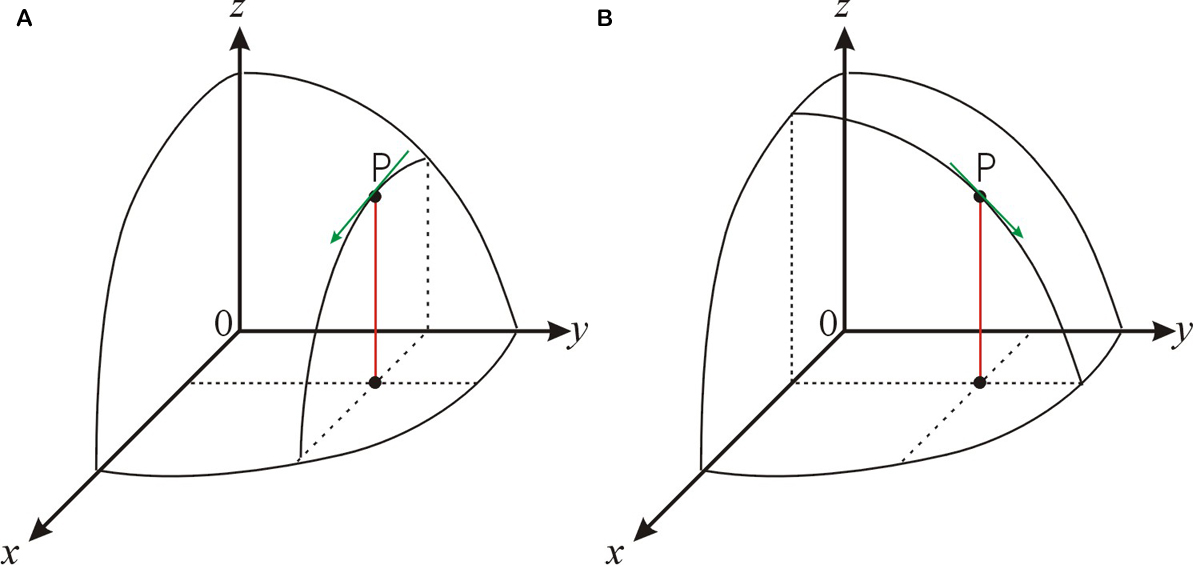
\includegraphics[width=0.8\linewidth]{02-partial}%
	\caption{Geometrický význam parciální derivace funkce v bodě \(P\).}%
	\label{fig:par}
\end{figure}

\begin{example}
	Mějme funkci \[f(x, y) = x^3 + 2xy - 15y\]
	Její parciální derivace v \(x\) je \[\frac{\partial f}{\partial x} (x, y) = 2x^2 + 2y\]
	a analogicky v \(y\) je \[\frac{\partial f}{\partial y} (x, y) = 2x - 15\]
\end{example}

\subsection{Totální diferenciál}
Nespojitá funkce $f$ může mít po souřadnicích všechny parciální derivace v každém bodě, to však ale neimplikuje spojitost.
\textbf{Existence parciálních derivací neimplikuje spojitost!}
Budeme potřebovat něco silnejšího. Připomeňme si tvrzení ekvivalentní se standardní derivací:

\begin{lemma}[Ekvivalentní definice derivace]
	Funkce \(f\) má v bodě \(x\) derivaci \(\iff\)  existuje $\mu$ konvergující k 0 při $h \rightarrow 0$ a A takové, že 
	\[f(x+h) - f(x) = Ah + |h| \cdot \mu(h)\]
\end{lemma}

\begin{intuition}
	$Ah + f(x) $ vyjadřuje tečnu ke grafu v bodě $(x,f(x))$ a $|h|\cdot \mu(h)$ je malá chyba\footnote{Je zajímavé si rozmyslet, proč vlastně násobíme \(|h|\) (jaké funkce budou mít derivace tam, kde by neměly).}, která je poměrově menší než \(|h|\), pro \(h \rightarrow 0\).
	Mysleme podobně o funkci $f(x,y)$ a uvažujme plochu:
	\[S = \{(t,u,f(t,u)) : (t,u) \in D\} \subseteq \mathbb{R}^3.\]
	Dvě parciální derivace vyjadřují směry dvou tečných přímek k S v bodě $(x,y,f(x,y))$, ale \textbf{ne tečnou rovinu},
	která teprve bude uspokojivé rozšíření faktu nahoře.
\end{intuition}

\subsubsection{Definice totálního diferenciálu}
Pro \textbf{x} $\in \mathbb{E}_n$ (místo absolutní hodnoty) definujeme \(||\textbf{x}||  = \max_i|x_i|\). $h$ bude $n$-tice blízká nule.

\begin{definition}[Totální diferenciál]
	Funkce $f$ má totální diferenciál v bodě \textbf{a}, existuje-li funkce $\mu$ spojitá v okolí $U$ bodu $\textbf{o} \in \mathbb{R}^n$ taková, že $\mu(\textbf{o}) = 0$
	a čísla $A_1,...,A_n$ pro která
	\[f(\textbf{a}+\textbf{h}) - f(\textbf{a}) = \sum^n_{k=1}A_kh_k+||\textbf{h}||\mu(\textbf{h}).\]
	S použitím skalárního součinu jde též zapsat jako
	$$f(\textbf{a} + \textbf{h}) - f(\textbf{a}) = \textbf{Ah} + ||\textbf{h}|| \mu (\textbf{h})$$
\end{definition}

\subsubsection{Věty o totálním diferenciálu}

\begin{lemma}[Spojitost, parciální derivace a totální diferenciál]\label{eq:satd}
	Nechť má funkce $f$ totální diferenciál v bodě \textbf{a}. Potom platí:
	\begin{enumerate}
	    \item $f$ je spojitá v \textbf{a},
	    \item $f$ má všechny parciální derivace v \textbf{a}, a to s hodnotami 
	    \[\frac{\partial f(\textbf{a})}{\partial x_k} = A_k.\]
	\end{enumerate}
\end{lemma}

\begin{proof}
	\begin{enumerate}
		\item Máme (dosazením do rovnice TD) \[|f(\textbf{x}) - f(\textbf{y})| \leq |\textbf{A}(\textbf{x}-\textbf{y})| + |\mu(\textbf{x}-\textbf{y})|\cdot||\textbf{x}-\textbf{y}||\]
		a limita na pravé straně pro \textbf{y} $\rightarrow$ \textbf{x} je 0.
		\item Máme (dosazením do rovnice TD) \[\frac{1}{h}(f(..., x_{k-1},x_k+h,x_{k+1},...) - f(x_1,...)) = A_k + \mu((...,0,h,0,...))\frac{||(0,...,h,...,0)||}{h},\]
		a limita na pravé straně je zřejmě $A_k$.
	\end{enumerate}
\end{proof}

Teď již spojitost dostaneme. Vidíme, že v případě funkcí jedné proměnné není rozdíl mezi existencí derivace v bodě \textbf{a} a vlastností
mít totální diferenciál v tomto bodě. V případě více proměnných je však tento rozdíl zcela zásadní. Může být trochu překvapující, že 
zatímco existence parciálních derivací mnoho neznamená, \textit{existence spojitých parciálních derivací} je něco úplně jiného.

\begin{theorem}[Spojité parciální derivace a totální diferenciál]
	Nechť má $f$ spojité parciální derivace v okolí bodu \textbf{a}. Potom má v \textbf{a} totální diferenciál.
\end{theorem}

\begin{proof}
	Buď
	\[\textbf{h}^{(0)} = \textbf{h}, \textbf{h}^{(1)} = (0, h_2,...,h_n), \textbf{h}^{(2)} = (0,0,h_3,...,h_n) \textrm{ atp.} \]
	(takže $\textbf{h}^{(n)} = \textbf{0})$.
	Potom máme
	\[f(\textbf{a}+\textbf{h}) - f(\textbf{a}) = \sum^n_{k=1}(f(\textbf{a}+\textbf{h}^{(k-1)})-f(\textbf{a}+\textbf{h}^{(k)})) = M.\]
	Podle Lagrangeovy věty \ref{lagrange1} existují $0 \leq \Theta_k \leq 1$ takové, že
	\[f(\textbf{a}+\textbf{h}^{(k-1)})-f(\textbf{a}+\textbf{h}^{(k)}) = \frac{\partial f(a_1,...,a_{k-1},a_k+ \Theta_kh_k,a_{k+1},...,a_n)}{\partial x_k}h_k\]
	a můžeme pokračovat
	\begin{align*} 
		\begin{split}
			M & = \sum\frac{\partial f(a_1,...a_k+\Theta_kh_k,...,a_n)}{\partial x_k}h_k = \\
			 & = \sum \frac{\partial f(\textbf{a})}{\partial x_k}h_k + \sum \left( \frac{\partial f(a_1,...,a_k+\Theta_kh_k,...,a_n)}{\partial x_k}
			 - \frac{\partial f(\textbf{a})}{\partial x_k} \right)h_k = \\
			 & = \sum \frac{\partial f(\textbf{a})}{\partial x_k}h_k + ||\textbf{h}||\sum\left(\frac{\partial f(a_1,...,a_k+\Theta_kh_k,...,a_n)}
			 {\partial x_k}- \frac{\partial f(\textbf{a})}{\partial x_k}\right)\frac{h_k}{||\textbf{h}||}.
		\end{split}
	\end{align*}
	Položíme
	\[\mu (\textbf{h}) =
	    \begin{cases} & \sum\left(\frac{\partial f(a_1,...,a_k+\Theta_kh_k,...,a_n)}{\partial x_k} -
	    \frac{\partial f(\textbf{a})}{\partial x_k} \right)\frac{h_k}{||\textbf{h}||}.\\
	    & 0 \text{ pokud } \mathbf{h} = \mathbf{o}
	    \end{cases}\]
	Jelikož $\left|\frac{h_k}{||\textbf{h}||}\right| \leq 1$ a jelikož jsou funkce $\frac{\partial f}{\partial x_k}$ spojité,
	$\lim_{\textbf{h}\rightarrow \textbf{0}} \mu (\textbf{h}) = 0$.
\end{proof}

\begin{consequence}
	Můžeme tedy schematicky psát \textbf{spojité PD $\implies$ TD $\implies$ PD}.
\end{consequence}


%%%%%%%%%%%%%%%%%%%%%%%%%%%%%%%%%%%%%%%%%%%%%%%%%%%%%%%%%%%%%%%%%%%%%%%%%%%%%%%%%%%%%%%%%%%%%%%%%%%%%%%%%
\subsection{Počítání parciálních derivací}
Aritmetická pravidla jsou stejná jako pro obyčejné derivace (tady totiž obyčejnými derivacemi jsou).
Trochu jinak tomu je u pravidla pro skládání. Pro derivace jedné proměnné se dokazuje z formule
\[ f(a+h) - f(a) = Ah + |h|\mu (h) \]
tedy z diferenciálu (který je pro ně totéž jako existence derivace).
Pravidlo pro skládání v nejjednodušší podobě následuje.

%%%%%%%%%%%%%%%%%%%%%%%%%%%%%%%%%%%%%%%%%%%%%%%%%%%%%%%%%%%%%%%%%%%%%%%%%%%%%%%%%%%%%%%%%%%%%%%%%%%%%%%%%
\subsubsection{Složené funkce}
\begin{theorem}[Derivace složených funkcí více proměnných]\label{th:dsf}
	Nechť má $f(\textbf{x})$ totální diferenciál v bodě \textbf{a}. Nechť mají $g_k(t)$ derivace v bodě $b$ a nechť je $g_k(b) = a_k$ pro 
	$k = 1,...n.$ Položme
	\[F(t) = f(\textbf{g}(t)) = f(g_1(t),...,g_n(t)).\]
	Potom má $F$ derivaci v $b$, totiž 
	\[F'(b) = \sum^n_{k=1}\frac{\partial f(\textbf{a})}{\partial x_k} \cdot g'_k(b).\]
\end{theorem}

\begin{proof}
	\begin{align*} 
	 \frac{1}{h} (F(b+h) - F(b)) &= \frac{1}{h}(f(\textbf{g}(b+h)) - f(\textbf{g}(b)) =  \\
	 &=\frac{1}{h}(f(\textbf{g}(b) + (\textbf{g}(b+h) - \textbf{g}(b))) - f(\textbf{g}(b)) = \\
	 &=\sum^n_{k=1}A_k\frac{g_k(b+h)-g_k(b)}{h} + \mu(\textbf{g}(b+h) - \textbf{g}(b)) \max_k\frac{|g_k(b+h)-g_k(b)|}{h}.
	\end{align*}
	Máme $\lim_{h \rightarrow 0} \mu(\textbf{g}(b+h)-\textbf{g}(b)) = 0$ jelikož jsou funkce $g_k$ spojité v $b$. 
	Jelikož funkce $g_k$ mají derivace, jsou $\max_k \frac{|g_k(b+h) - g_k(b)|}{h}$ omezené v dostatečně malém okolí nuly. Limita 
	poslední sčítance je tedy nula a máme
	\[
		\begin{aligned}
			F'(b) &= \lim_{h \rightarrow 0} \frac{1}{h}(F(b+h) - F(b)) \\
			&= \lim_{h \rightarrow 0} \sum^n_{k = 1} A_k\frac{g_k(b+h)-g_k(b)}{h} \\
			&= \sum^n_{k = 1}A_k\lim_{h \rightarrow 0} \frac{g_k(b+h) - g_k(b)}{h} \\
			&= \sum^n_{k = 1}\frac{\partial f(\textbf{a})}{\partial x_k}g'_k(b)
		\end{aligned}
	\]

	Kde v poslední rovnosti využíváme tvrzení \ref{eq:satd}, díky kterému $A_k = \frac{\partial f(\textbf{a})}{\partial x_k}$.
\end{proof}

\begin{intuition}
	Tečná nadrovina vyjádřená diferenciálem vnější funkce $f$ nemá žádný důvod preferovat hlavní osy, v nichž se 
	dějí derivace vnitřních funkcí. Proto by tady jen parciální derivace nestačily.
\end{intuition}

\begin{theorem}[Řetízkové Pravidlo]
	Nechť má $f(\textbf{x})$ \textit{totální diferenciál} v bodě \textbf{a}. Nechť mají funkce $g_k(t_1,...,t_r)$ parciální 
	derivace v \textbf{b} $= (b_1,...,b_r)$ a nechť je $g_k(\textbf{b}) = a_k$ pro $k = 1,...,n.$ Potom má funkce
	\[(f\circ \textbf{g})(t_1,...,t_r) = f(\textbf{g}(t)) = f(g_1(t),...,g_n(t))\]
	všechny parciální derivace v \textbf{b}, a platí 
	\[\frac{\partial (f \circ \textbf{g})(\textbf{b})}{\partial t_j} = \sum^n_{k=1}\frac{\partial f(\textbf{a})}{\partial x_k}
	\cdot \frac{\partial g_k(\textbf{b})}{\partial t_j}.\]
\end{theorem}

\begin{proof}
	Skládali jsme
	\[\mathbb{E}_k \xrightarrow{\mathbf{g}} \mathbb{E}_n \xrightarrow{\textit{f}} \mathbb{R} \]
	Skládejme místo $f$ $m$-tici funkcí
	$\mathbf{f} = (f_1,...,f_m)$, tedy $\mathbf{f}: \mathbb{E}_n \rightarrow \mathbb{E}_m$
	\[\mathbb{E}_k \xrightarrow{\mathbf{g}} \mathbb{E}_n \xrightarrow{\textit{f}} \mathbb{E}_m \]
	Pravidlo z předchozí věty dá tedy
	\[\frac{\partial (f_i \circ \mathbf{g})(b)}{\partial t_j} = \sum^n_{k=1} \frac{\partial f_i(\mathbf{a})}{\partial x_k}
	\cdot \frac{\partial g_k(\mathbf{b})}{\partial t_j}.\]
\end{proof}

\begin{remark}
	Zavedeme-li matice $D\mathbf{f} = \left(\frac{\partial f_i(\mathbf{a})}{\partial x_k}\right)_{ik}$ je 
	$D(\mathbf{f}\circ \mathbf{g}) = D\mathbf{f}\cdot D\mathbf{g}$ (napravo násobení matic), a tak to má být. $D\mathbf{h}$ je matice lineární aproximace 
	funkce $\mathbf{h}$: \textit{lineární aproximace se skládají spolu s aproximovanými funkcemi}.
\end{remark}

\subsubsection{Násobení}
\[ f(u,v) = u \cdot v \]

Potom $ \frac{\partial f}{\partial u} = v $ a $ \frac{\partial f}{\partial v} = u $
a pro $u = \psi (x)$ a $ v = \phi (x) $ platí:
\[ (\phi (x) \psi (y))' =
\frac{\partial f}{\partial u} \phi '(x) + \frac{\partial f}{\partial v} \psi '(x) = 
\phi (x)\psi '(x) + \phi '(x)\psi (x)  \]

%%%%%%%%%%%%%%%%%%%%%%%%%%%%%%%%%%%%%%%%%%%%%%%%%%%%%%%%%%%%%%%%%%%%%%%%%%%%%%%%%%%%%%%%%%%%%%%%%%%%%%%%%%
\subsubsection{Dělení}
\[ f(u,v) = \frac{u}{v} \]

Potom $ \frac{\partial f}{\partial u} = \frac{1}{v} $ a $ \frac{\partial f}{\partial v} = -\frac{u}{v^2} $
a pro $u = \psi (x)$ a $ v = \phi (x) $ platí:
\[ \left( \frac{\phi (x)}{\psi (x)} \right)' =
\frac{\partial f}{\partial u} \phi '(x) - \frac{\partial f}{\partial v} \psi '(x) =
\frac{1}{\psi (x)} \phi '(x) + \frac{1}{\psi (x)^2}\psi '(x) =
\frac{\psi (x)\phi '(x) - \phi (x)\psi '(x)}{\psi (x)^2} \]

\subsection{Lagrangeovy věty}
\begin{definition}[Konvexní množina]
	Podmnožina $U \subseteq \mathrm{E}_n$ je konvexní, pokud
	$$\forall \mathbf{x}, \mathbf{y} \in U \quad \implies \quad \forall t, 0 \le t \le 1, (1 - t) \mathbf{x} + t \mathbf{y} = \mathbf{x} + t( \mathbf{y} - \mathbf{x}) \in U$$
\end{definition}

\begin{figure}[h]
	\centering
	\subfloat[\centering Konvexní]{{\includegraphics[width=5cm]{02.convex} }}%
	\hspace{5em}
	\subfloat[\centering Nekonvexní]{{\includegraphics[width=5cm]{02.non-convex} }}%
	\caption{Příklad konvexní a nekonvexní podmnožiny $\mathrm{E}_n$}%
\end{figure}

\begin{theorem}[Lagrangeova věta v jedné proměnné]
	Nechť $f$ je spojitá funkce na intervalu $[a, b]$ a má na $(a, b)$ derivaci. Pak existuje bod $c \in (a, b)$ t. ž. tečna v bodě $c$ je rovná přímce procházející $(a, f(a))$ a $(b, f(b))$: $$f'(c) = \frac{f(b) - f(a)}{b - a} \qquad \text{nebo ekvivalentně} \qquad f(b) - f(a) = f'(c)(b - a)$$
\end{theorem}

\begin{figure}[h]
	\centering
	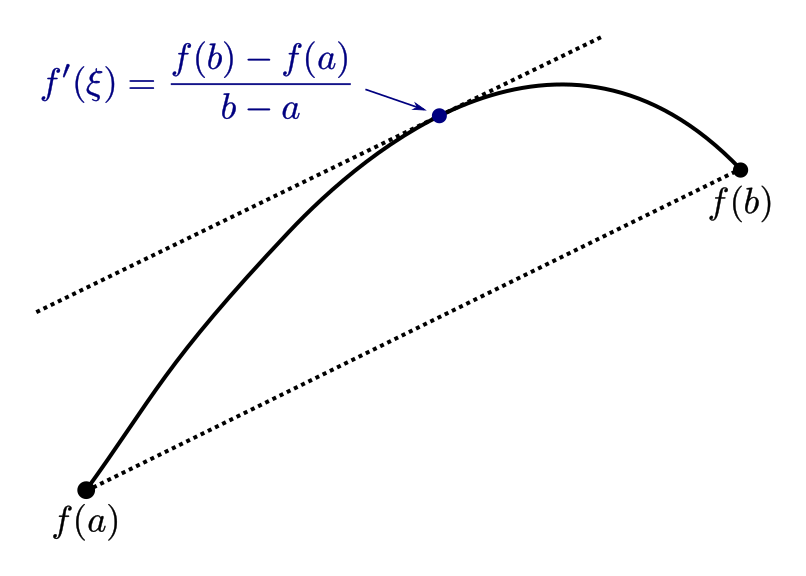
\includegraphics[width=0.5\linewidth]{02-lagrange}%
	\caption{Geometrický význam Lagrangeovy věty v jedné proměnné.}%
	\label{fig:par}
\end{figure}

\begin{theorem}[Lagrangeova věta ve více proměnných]\label{lagrange1}
	Nechť má $f$ spojité parciální derivace v konvexní otevřené množině $U \subseteq \mathbb{E}_{n}$.
	Potom pro libovolné dva body $x,y \in U$ $\exists 0 \leq \theta \leq 1$ takové, že:
	\[ f(\mathbf{y}) - f(\mathbf{x}) = \sum^{n}_{j=1} \frac{\partial f(\mathbf{x} + \theta (\mathbf{y}-\mathbf{x}))}{\partial x_j}(y_j - x_j) \]
	nebo ekvivalentně jako
	\[ f(\mathbf{y}) - f(\mathbf{x}) = \Delta f(\textbf{c}) (\textbf{y} - \textbf{x}) \]
	kde \(\textbf{c} = \mathbf{x} + \theta (\mathbf{y}-\mathbf{x})\) a \[\Delta f(p) = \begin{pmatrix} \frac{\partial f}{\partial x_1} \\[6pt] \vdots \\[6pt] \frac{\partial f}{\partial x_n} \end{pmatrix}\] je \textbf{gradient} funkce \(f\).
\end{theorem}

\begin{intuition}
	Jedná se o přímočaré zobecnění Lagrangeovy věty pro více proměnných, kde derivaci zobecňujeme gradientem (geometricky opět vektor tečné nadroviny v daném bodě) a skalárním součinem.
\end{intuition}

\begin{proof}
	Položme $F(t) = f(\mathbf{x} + t(\mathbf{y} - \mathbf{x}))$ a $\mathbf{g}$ t. ž. $g_j(t) = x_j + t(y_j - x_j)$.
	Potom máme $F(t) = f \circ \mathbf{g} = f(\mathbf{x} + t(\mathbf{y}-\mathbf{x}))$ a
	\[ F'(t) = \sum^{n}_{j=1} \frac{\partial f(\mathbf{g}(t))}{\partial x_j}g_j'(t) =
	\sum^{n}_{j=1} \frac{\partial f(\mathbf{g}(t))}{\partial x_j}(y_j - x_j)  \]
	Podle Lagrangeovy věty $\exists \theta : 0 \leq \theta \leq 1$ a díky tomu, že $f(\mathbf{x}) = F(0)$ a $f(\mathbf{y}) = F(1)$ dostáváme:
	\[ f(\mathbf{y}) - f(\mathbf{x}) = F(1) - F(0) = F'(\theta)(1 - 0) = F'(\theta) \]
\end{proof}


\begin{remark}
	Často se užívá v tomto tvaru (porovnej s formulí pro totální diferenciál):
	\[ f(\mathbf{x} + \mathbf{h}) - f(\mathbf{x}) =
	\sum^{n}_{j=1} \frac{\partial f(\mathbf{x + \theta \mathbf{h}})}{\partial x_j}h_j \]
\end{remark}

\subsection{Záměnnost pořadí při parciálních derivacích}
\begin{lemma}[O záměnnosti]
	Mějme funkci $f(x,y)$ takovou, že existují parciální derivace
	$\frac{\partial ^2 f}{\partial x \partial y}$ a $\frac{\partial ^2 f}{\partial y \partial x}$, které
	jsou spojité v nějakém okolí bodu $(x,y)$. Potom:
	\[ \frac{\partial ^2 f(x,y)}{\partial x \partial y} = \frac{\partial ^2 f(x,y)}{\partial y \partial x} \]
\end{lemma}

\begin{proof}
	Pokusíme se spočíst obě derivace v jednom kroku, tedy počítejme limitu $\lim_{h\rightarrow 0} F(h)$ funkce
	\[F(h) = \frac{f(x+h,y+h) - f(x,y+h) - f(x+h,y) + f(x,y)}{h^2}\]
	Položíme-li 
	\begin{align*} 
		\begin{split}
			\varphi_h(y) & = f(x+h,y) - f(x,y)\text{ a}\\
			\psi_h(x) & = f(x,y+h) - f(x,y),
		\end{split}
	\end{align*}
	dostaneme pro $F(h)$ dva výrazy:
	\begin{align*} 
		\begin{split}
			F(h) & = \frac{1}{h^2} (\varphi_h(y+h) - \varphi_h(y))\\
			F(h) & = \frac{1}{h^2} (\psi_h(x+h)-\psi_h(x)).
		\end{split}
	\end{align*}
	První: Funkce $\varphi_h$ má derivaci (podle $y$, jinou proměnnou nemá)
	\[\varphi'_h(y)=\frac{\partial f(x+h,y)}{\partial y}-\frac{\partial f(x,y)}{\partial y}\]
	a tedy podle Lagrangeovy věty \ref{lagrange1} (druhý tvar, rozdíl je $y + h - y = h$):
	\begin{align*}
		F(h) & = \frac{1}{h^2}(\varphi_h(y+h)-\varphi_h(y)) = \frac{1}{h}\varphi'_h(y+\theta_1h)\\
		& = \frac{\partial f(x+h,y+\theta_1h)}{\partial y} -\frac{\partial f(x,y+\theta_1h)}{\partial y}.
	\end{align*}
	Potom znovu podle Lagrangeovy věty 
	\[F(h) = \frac{\partial }{\partial x}\left(\frac{\partial f(x+\theta_2h,y+\theta_1h}{\partial y}\right)\]
	pro nějaká $\theta_1,\theta_2$ mezi 0 a 1.
	Druhá, $\frac{1}{h^2}(\varphi_h(x+h) - \varphi_h(x)))$ dá podobně
	\[F(h) = \frac{\partial }{\partial y}\left(\frac{\partial f(x+\theta_4h,y + \theta_3h}{\partial x}\right)\]
	Obě $\frac{\partial }{\partial y}(\frac{\partial f}{\partial x})$ a $\frac{\partial }{\partial x}(\frac{\partial f}{\partial y})$ jsou spojité ($x,y$), a $\lim_{h\rightarrow 0} F(h)$ můžeme počítat z kteréhokoli výrazu (první nebo druhá):
	\[\lim_{h\rightarrow 0}F(h) = \frac{\partial ^2 f(x,y)}{\partial x \partial y} 
	                            = \frac{\partial ^2 f(x,y)}{\partial y \partial x}.\]
\end{proof}

\begin{consequence}
	Nechť má funkce $f$ v proměnných spojité parciální derivace do řádu $k$. Potom hodnoty těchto derivací
	záleží pouze na tom, kolikrát bylo derivováno v každé z proměnných $x_1, ... , x_n$.
	Tedy za daných předpokladů můžeme obecné parciální derivace řádu $r \leq k$ psát
	\[\frac{\partial ^r f}{\partial x^{r_1}_1 \partial x^{r_2}_2 ... \partial x_n^{r_n}} \text{ kde } r_1 + r_2 + \cdot \cdot \cdot + r_n = r \]
	\[(r_j = 0 \text{ indukuje absenci symbolu } \partial x_j)\]
\end{consequence}

\subsection{Věta o konvergentní podposloupnosti}
\begin{theorem}[Konvergentní podposloupnost na kompaktním intervalu]
	Mějme $a,b \in \mathbb{R}$ taková, že $\forall n: a \leq x_n \leq b$. Potom existuje podposloupnost
	$(x_{k_n})_n$ posloupnosti $(x_n)_n$ která konverguje v $\mathbb{R}$ a platí
	$a \leq \lim_n x_{k_n} \leq b$
\end{theorem}

\begin{proof}
	Vezměme \[M = \{x : x \in \mathbb{R}, x \leq x_n \text{ pro nekonečně mnoho n}\}\]
	$M$ je neprázdná a omezená protože $a \in M \text{ a } b$ je horní mez $M$. Musí tedy existovat $s = sup(M)$ a platí 
	$a \leq s \leq b$. Dále, pro každé $n$ je množina 
	\[K(n) = \left\{k : s - \frac{1}{n} < x_k < s + \frac{1}{n}\right\}\]
	nekonečná: skutečně, máme $x > s - \varepsilon$ takové, že $x_n > x$ pro nekonečně mnoho $n$, zatím co podle definice množiny M je jen
	konečně mnoho $n$ takových, že $x_n \geq s + \varepsilon$. 
	Zvolme $k_1$ tak, aby
	\[s - 1 < x_{k_{1}} < s+1.\]
	Mějme zvolena $k_1 < k_2 < \cdot \cdot \cdot < k_n$ taková, že $j = 1,...,n$
	\[s - \frac{1}{j} < x_{k_j} < s + \frac{1}{j}.\]
	Jelikož $K(n+1)$ je nekonečná, můžeme zvolit $k_{n+1} > k_n$ tak, aby
	\[s - \frac{1}{n+1} < x_{k_{n+1}} < s + \frac{1}{n+1}.\]
	Takto zvolená podposloupnost $(x_{k_n})_n$ naší $(x_n)_n$ zřejmě konverguje k $s$.
\end{proof}

\end{document}
